\documentclass[../report.tex]{subfiles}

\begin{document}
\graphicspath{{img/}{../img/}}

This section is dedicated to explain the architecture behind \textit{Artshare}, which is the client of this system, developed to use the ShareIt services. \textit{ArtShare} has been developed using the ASP.NET MVC framework by Microsoft\footnote{http://www.asp.net/mvc}. 

%The students at SMU developed another client using the functionality of the server, but the architecture of this client will not be described in this section nor in this report.

\subsection{ASP.NET MVC}

The ASP.NET MVC framework implements, as the name suggest, the model-view-controller architectural pattern, denoted by the abbreviation MVC. This pattern divides applications into three main components which seperates application data and logic from the view that is displayed to the user. 

In MVC the model represents the application domain data, which is the core part of the application. Most often the model objects are used to retrieve and store objects in a database. The view is a representation of data and is displayed to the user. The controller is what the user interacts with to manipulate the data objects. It reads data and user input from the view and sends the manipulated data to the model. The controller also selects which view to render and passes on a specfic model if this is necessary.

\begin{figure}[H]
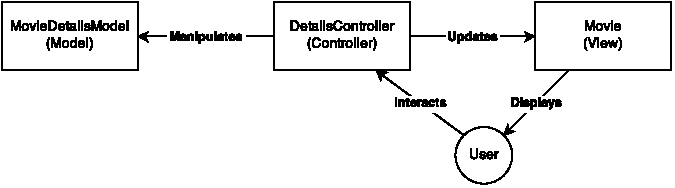
\includegraphics[width=\linewidth]{mvc.pdf}
\caption{Example of MVC use in ArtShare}
\label{fig:mvc}
\end{figure}

Figure \ref{fig:mvc} shows an example of how MVC components interact with each other, using an actual example from Artshare. The figure illustrates the interaction when movie details are shown. A user interacts with ArtShare and asks for the movie details of a movie with a specific id. The controller manipulates the model, such that the model contains data about the correct movie. The controller then updates the view, by passing the manipulated model to the view, which is then displayed to the user.

The controllers in ArtShare delegate most of their tasks to the logic classes, which are interfaced. This allows for easier testing of the controllers and makes the logic classes replaceable if at one point it is decided to use a different logic (for instance a logic using a different service). The controller classes have overloaded constructors in order to support the injection of a logic class. The following code-snippet shows how this is done in the DetailsController class.

\begin{lstlisting}
	private readonly IDetailsLogic _logic;
	public DetailsController() {
		_logic = new DetailsLogic();
	}
	public DetailsController(IDetailsLogic detailsLogic) {
		_logic = detailsLogic;
	}
\end{lstlisting}

%In MVC the model represents the application domain data, which is the core part of the application. Most often the model objects are used to retrieve and store objects in a database. In ArtShare the model is defining all properties, determining which data to be used by a view.

%A view is a representation of data that is displayed to the user, therefore views are the UI of the application. All views are populated with the data objects defined in the model. The controller is what the user interacts with to manipulate the data objects in the model. It reads data and user input from the view and sends the manipulated data to the model. The controller also selects which view to render and passes on a specfic model if this is necessary.


\subsection{Motivation}

\paragraph{Motivation for choosing MVC}
When developing front-end you can choose between numerous great frameworks and development patterns. ASP.NET offers three patterns, where MVC is one of them. The seperation of the application components in MVC ensures a loose coupling, which is the key motivation for choosing this framework.

Especially the seperation of the application data is a relevant part when talking about the development of ArtShare. The models developed are used in several views in the application. An example is the detailmodels\footnote{MovieDetailsModel, MusicDetailsModel, BookDetailsModel}, which are used to display, edit and upload \textit{Media Items}.

The loose coupling in the application framework also forms a sound basis for parallel programming. When the model has been implemented, the developers can simultaneously work on the controllers and the views.

Specifically ASP.NET MVC uses a Front-controller pattern to process requests through a single controller. This means that you are able to control all routings of the application. There has been made use of this in ArtShare to simplify paths and make the details page more generic, so that \texttt{/details/\{id\}} will reroute to \texttt{/details/movie/\{id\}} if the given id is a movie.

\paragraph{Motivation for choosing .NET}
Lots of powerful Javascript frameworks offer to develop web applications in MVC. Some of the most used are Angular.js, Backbone.js and Knockout.js. Other languages such as Ruby on Rails also uses MVC, like most of the web frameworks that exists.

Since the server is developed using the .NET platform it was an obvious choice to also develop the client in a .NET platform. The server provides services through service references. Using ASP.NET MVC, which is a .NET platform, it was easy to use these services, just by referencing them in the \texttt{web.config} file. 

\subsection{Upload \& Download}

The possibility to upload and download \textit{Media Items} in ArtShare, is one of the most vital features of a system where sharing media is the focal point. From the functional requirement FR-39, we have that a \textit{User} must be able to upload media items, while FR-45, FR-46 and FR-47 explains that a User must be able to download media items, if certain conditions are fulfilled.

In ArtShare upload-functionality is provided to the users through different types of input fields. By using the HTML file type attribute\footnote{http://www.w3schools.com/tags/att\_input\_type.asp} on an input field, users are able to select files using their native file system. The file is, along with information on the media file, posted to the UploadController which invokes a method on the service.

When a User wants to download a media item, a method in the DownloadController is called. The DownloadController request the correct media item, by invoking a service exploited by ShareIT. The service returns a stream, which is then divided into small pieces before it is returned in a HTTP result. The reason for this breakdown of the stream is to ensure that the stream doesn't exceed the maximum buffer limit on the client. This design choice can also be traced back to NFR-06, namely that ArtShare must be able to support 10 concurrent users. Depending on the user's browser, the returned stream can be handled in various ways. E.g. when the browser Chrome (v31+) receives an HTTP result containing a stream, it automatically initiates the download process.



\end{document}